% Provenance (never printed): see sources/outline_sources.md (Year 1: compaction and
% cementation; basin types; subsidence, accommodation and sea-level change). Exercise and
% problem values in the Book 3 scratch calculator calc/ch23.py; figure data from
% figdata/bachelor-1/compaction.py and sea_level.py.
% Porosity and permeability are Book 1's (g6); diagenesis was met in Book 2 (g12) and is
% re-founded here; sedimentary basin was met in Book 2 (g11) and is re-founded here;
% isostasy and the equal-mass proposition are ch. 11's; passive margins and rifts ch. 13's;
% effective stress ch. 16's; the Last Glacial Maximum and glacial cycles Book 2's (g12).
% Pressure solution is defined in the Year 3 volume (deformation mechanisms): prose only.
% Backstripping, the stretching model and the comparison of basins are the Year 2 volume's.
\chapter{Diagenesis and Sedimentary Basins}\label{ch:b1:diagenesis-basins}

Beach sand is loose: half of it, by volume, is water between the grains. Buried
three kilometres down, the same sand comes back up in a drill core as hard
sandstone, its grains pressed together and the space between them much reduced
and partly filled with new quartz. Between the beach and the core lie millions of years in which
the sediment was buried under more sediment, squeezed, heated and soaked in
water that dissolved some \omterm{def:b1:rock-forming-minerals:mineral}{minerals} and laid down others. This chapter follows
those changes, then steps back to the places where sediment can pile up
kilometres thick --- the \omterm{def:b1:diagenesis-basins:basin}{sedimentary basins} --- and to the two things that make
room for it there: the sinking of the floor, and the rise and fall of the sea.

\begin{recall}
The porosity of a rock is the fraction of its volume made of pores, and its
permeability measures how easily water flows through them (Book~1, grade~6).
A region is in \omterm{def:b1:isostasy-gravity:isostasy}{isostasy} when every column down to the \omterm{def:b1:isostasy-gravity:isostasy}{compensation depth} holds
the same mass (\cref{prop:b1:isostasy-gravity:equal-mass}). Rifts open by normal
faulting, and \omterm{def:b1:rifts-ridges-margins:passive-margin}{passive margins} are the edges of continents left behind when a
rift becomes an ocean (\cref{ch:b1:rifts-ridges-margins}). The \omterm{def:b1:stress-strain-rheology:lithostatic}{effective stress}
is the stress minus the \omterm{def:b1:stress-strain-rheology:lithostatic}{pore-fluid pressure}
(\cref{def:b1:stress-strain-rheology:lithostatic}). The last glacial cycle
reached its Last Glacial Maximum some twenty thousand years ago (Book~2,
grade~12). Sandstones, shales and their environments are those of
\cref{ch:b1:clastic-sediments}; limestones, chalk, dolomite and \omterm{def:b1:chemical-biogenic-sediments:evaporite}{evaporites} those
of \cref{ch:b1:chemical-biogenic-sediments}.
\end{recall}

\section{Compaction}\label{sec:b1:diagenesis-basins:compaction}

A sediment newly laid down is a loose packing of grains with water in between.
Everything that happens to it after deposition and before metamorphism, while it
stays at the low temperatures and pressures of the upper few kilometres of the
\omterm{def:b1:layered-earth:layers}{crust}, belongs to one family of processes.

\begin{definition}[Diagenesis]\label{def:b1:diagenesis-basins:diagenesis}
\emph{Diagenesis}\index{diagenesis} is the set of physical, chemical and
biological changes that a sediment undergoes after its deposition, at the
temperatures and pressures of the upper \omterm{def:b1:layered-earth:layers}{crust}, below those of metamorphism. It
includes \omterm{def:b1:diagenesis-basins:compaction}{compaction}, \omterm{def:b1:diagenesis-basins:cement}{cementation}, the dissolution of grains, and the
replacement of one \omterm{def:b1:rock-forming-minerals:mineral}{mineral} by another; together they turn a loose sediment into
a sedimentary rock.
\end{definition}

The first of these changes is mechanical. Each new layer adds its weight to
those below. The grains are pressed together, slide and rotate into a tighter
packing, the soft ones (clay flakes, rock fragments, \omterm{def:b1:rock-forming-minerals:groups}{mica}) bend between the hard
ones, and the water between them is driven out.
% ledger: og:diagenesis

\begin{definition}[Compaction, decompaction]\label{def:b1:diagenesis-basins:compaction}
\emph{Compaction}\index{compaction} is the loss of volume of a sediment under
the weight of the sediments above it, by the closer packing of its grains, the
expulsion of its pore water and, deeper, the dissolution of grains where they
touch. \emph{Decompaction}\index{decompaction} is the calculation that restores
a buried layer to the thickness it had at an earlier, shallower burial, most
often at the surface, when it was laid down.
\end{definition}

Porosities measured in wells fall with depth, steeply near the surface and then
more and more slowly. In 1930 L.~F. Athy fitted them with an exponential, and
the fit has been the starting point of \omterm{def:b1:diagenesis-basins:compaction}{compaction} studies ever since.
% ledger: sc80:athy

\begin{proposition}[Athy's law]\label{prop:b1:diagenesis-basins:athy}
In a pile of sediment of one lithology, compacted under its own weight with its
pore water free to escape, the porosity at the depth $z$ below the surface is
\[
  \varphi(z) = \varphi_0\, e^{-z/\lambda},
\]
where $\varphi_0$, the surface porosity, and $\lambda$, the decay length, depend
on the lithology. This is \emph{Athy's law}\index{Athy's law}.
\end{proposition}
\admitted

The law is an empirical fit, not a consequence of theory. Its parameters are
measured, lithology by lithology, from the porosities of wells; the values of
\cref{tab:b1:diagenesis-basins:athy}, published with a study of the \omterm{def:b1:diagenesis-basins:subsidence}{subsidence}
of the North Sea, are widely used to correct for \omterm{def:b1:diagenesis-basins:compaction}{compaction}. Shale starts with more water than sand
but loses it over a shorter distance; chalk, the most porous of the three at the
surface, loses it fastest of all. At \qty{3000}{m} the law gives a porosity of
\num{0.22} for sandstone, \num{0.14} for shale and \num{0.08} for chalk (figure
below): the sand of the opening has lost more than half its pores.
% ledger: pybacktrack:compaction, sc80:north-sea

\begin{table}[htbp]
\centering
\begin{tabular}{lccc}
\hline
lithology & surface porosity $\varphi_0$ & decay length $\lambda$ (m) & grain density (\unit{kg.m^{-3}}) \\
\hline
shale            & 0.63 & 1960 & 2700 \\
sandstone        & 0.49 & 3704 & 2650 \\
shaly sandstone  & 0.56 & 2564 & 2680 \\
chalk            & 0.70 & 1408 & 2710 \\
\hline
\end{tabular}
\caption{The parameters of \omterm{prop:b1:diagenesis-basins:athy}{Athy's law} and the densities of the grains for four
lithologies, after Sclater and Christie (1980), as tabulated in the open
backtracking software pyBacktrack.}
\label{tab:b1:diagenesis-basins:athy}
\end{table}
% ledger: pybacktrack:compaction

\omterm{def:b1:diagenesis-basins:compaction}{Compaction} squeezes out water; it neither adds grains nor takes them away, as
long as nothing is dissolved and carried off or brought in as \omterm{def:b1:diagenesis-basins:cement}{cement}. The volume
of the grains in a column is therefore the quantity to follow as the column is
buried.

\begin{proposition}[Solid thickness of a layer]\label{prop:b1:diagenesis-basins:solid}
Under \omterm{prop:b1:diagenesis-basins:athy}{Athy's law}, a layer between the depths $z_1 < z_2$ holds, per unit area, a
volume of grains equal to the thickness
\[
  s = (z_2 - z_1) - \varphi_0 \lambda \left( e^{-z_1/\lambda} - e^{-z_2/\lambda} \right).
\]
If the layer is moved to a new depth without loss or gain of grains, its new top
$z_1'$ and bottom $z_2'$ satisfy $s(z_1', z_2') = s(z_1, z_2)$, and for a given
$z_1'$ this equation has exactly one solution $z_2'$.
\end{proposition}

\begin{proof}
A slice of thickness $\mathrm dz$ at the depth $z$ contains the volume of grains
$(1 - \varphi(z))\,\mathrm dz$ per unit area. Integrating from $z_1$ to $z_2$,
\[
  s = \int_{z_1}^{z_2} \bigl(1 - \varphi_0 e^{-z/\lambda}\bigr)\,\mathrm dz
    = (z_2 - z_1) - \varphi_0\lambda\left(e^{-z_1/\lambda} - e^{-z_2/\lambda}\right).
\]
With the top fixed at $z_1'$, the function $f(b) = s(z_1', b)$ has the
derivative $1 - \varphi(b) > 0$, since a porosity is less than one; it is
continuous, zero at $b = z_1'$ and grows without bound, so it takes the value
$s(z_1, z_2)$ exactly once.
\end{proof}

\begin{method}[Decompacting a layer]\label{met:b1:diagenesis-basins:decompaction}
\begin{enumerate}
  \item Read the top $z_1$ and the bottom $z_2$ of the layer today, and its
        parameters $\varphi_0$ and $\lambda$
        (\cref{tab:b1:diagenesis-basins:athy}).
  \item Compute its solid thickness $s$ with
        \cref{prop:b1:diagenesis-basins:solid}.
  \item Choose the depth $z_1'$ of its top at the earlier time --- zero to
        restore it to the surface.
  \item Solve $s(z_1', b) = s$ for the new bottom $b$ by Newton's method:
        start from $b_0 = z_1' + (z_2 - z_1)$ and repeat
        \[
          b_{k+1} = b_k - \frac{s(z_1', b_k) - s}{1 - \varphi(b_k)}
        \]
        until the change is below the precision wanted; two or three steps are
        usually enough.
  \item The thickness of the layer at that time is $b - z_1'$; its mean
        porosity is $1 - s/(b - z_1')$.
\end{enumerate}
\end{method}

Take \qty{500}{m} of shale between \qty{3000}{m} and \qty{3500}{m}. It holds
\qty{440}{m} of grains and only \qty{60}{m} of water, a mean porosity of
\num{0.12}. Brought back to the surface, the same grains make a layer
\qty{891}{m} thick, half of it water (figure below). The thickness of a buried
shale is barely more than half of what was laid down; rates of sedimentation
read from buried sections must be decompacted before they are compared with
rates measured today.
% computed in figdata/bachelor-1/compaction.py; ledger: pybacktrack:compaction

\begin{omfigure}
\begin{tikzpicture}[font=\footnotesize]
\begin{axis}[name=phi, width=7.6cm, height=7.2cm, xmin=0, xmax=0.75, ymin=0, ymax=5000,
    y dir=reverse, xlabel={porosity $\varphi$}, ylabel={depth (m)},
    xtick={0,0.2,0.4,0.6}, ytick={0,1000,...,5000},
    legend style={at={(0.97,0.03)}, anchor=south east, font=\scriptsize, draw=none, fill=white, fill opacity=0.85, text opacity=1},
    legend cell align=left]
  \addplot[thick, omLithSand!50!black] table[x=phi_sand, y=z] {figdata/out/bachelor-1-compaction-curves.dat};
  \addplot[thick, omThm, densely dashed] table[x=phi_shale, y=z] {figdata/out/bachelor-1-compaction-curves.dat};
  \addplot[thick, omLithLime!50!black, dash dot] table[x=phi_chalk, y=z] {figdata/out/bachelor-1-compaction-curves.dat};
  \legend{sandstone, shale, chalk}
  \draw[black!50, dotted] (axis cs:0,3000) -- (axis cs:0.75,3000);
\end{axis}
\begin{axis}[at={(phi.east)}, anchor=west, xshift=1.6cm, width=6.4cm, height=7.2cm,
    ybar stacked, bar width=1.1cm, ymin=0, ymax=1000, enlarge x limits=0.45,
    symbolic x coords={buried, surface}, xtick=data,
    xticklabels={{at 3000--3500 m}, {at the surface}},
    ylabel={thickness of the layer (m)}, ytick={0,200,...,1000},
    legend style={at={(0.03,0.97)}, anchor=north west, font=\scriptsize, draw=none},
    legend cell align=left]
  \addplot[fill=omLithShale, draw=black!60] table[x=state, y=solid] {figdata/out/bachelor-1-compaction-demo.dat};
  \addplot[fill=omSea, draw=black!60] table[x=state, y=pore] {figdata/out/bachelor-1-compaction-demo.dat};
  \legend{grains, pore water}
  \node[anchor=south] at (axis cs:buried,500) {\qty{500}{m}};
  \node[anchor=south] at (axis cs:surface,891) {\qty{891}{m}};
\end{axis}
\end{tikzpicture}

{\small Left: porosity against depth by \omterm{prop:b1:diagenesis-basins:athy}{Athy's law} for sandstone, shale and
chalk, with the parameters of \cref{tab:b1:diagenesis-basins:athy}. Right:
\qty{500}{m} of shale between \qty{3000}{m} and \qty{3500}{m}, and the same
layer decompacted to the surface: the grains (\qty{440}{m}) are kept, the water
is not.}
\label{fig:b1:diagenesis-basins:compaction}
\end{omfigure}
% computed in figdata/bachelor-1/compaction.py; ledger: pybacktrack:compaction

\omterm{prop:b1:diagenesis-basins:athy}{Athy's law} holds only while the water can leave. \omterm{def:b1:diagenesis-basins:compaction}{Compaction} is driven by the
\omterm{def:b1:stress-strain-rheology:lithostatic}{effective stress}, the weight of the rock above minus the pressure of the water
in the pores (\cref{ch:b1:stress-strain-rheology}). Where a thick shale is buried
faster than its water can seep out, the water carries part of the load, the pore
pressure rises above the hydrostatic, and the shale keeps a porosity too high for
its depth: it is overpressured, and the correction for \omterm{def:b1:diagenesis-basins:compaction}{compaction} must allow for
it.
% ledger: sc80:north-sea

Deeper, \omterm{def:b1:diagenesis-basins:compaction}{compaction} becomes chemical. Where two quartz grains press on each
other through a film of water, and especially where a flake of clay or \omterm{def:b1:rock-forming-minerals:groups}{mica} lies
between them, quartz dissolves at the contact; the silica diffuses a short way
through the water and is laid down again on clean quartz surfaces facing the
open pores. The grains interpenetrate, and dissolution concentrated along
surfaces leaves stylolites, jagged seams of the insoluble residue. This pressure
solution, which the Year~3 volume treats as a mechanism of deformation, is both
the last stage of \omterm{def:b1:diagenesis-basins:compaction}{compaction} and the source of the commonest \omterm{def:b1:diagenesis-basins:cement}{cement} of
sandstones.
% ledger: walderhaug:quartz, oye:quartz-cement

\section{Cementation and other changes}\label{sec:b1:diagenesis-basins:cementation}

\omterm{def:b1:diagenesis-basins:compaction}{Compaction} alone makes a dense sediment, not a hard rock. The grains are glued
into a rock by \omterm{def:b1:rock-forming-minerals:mineral}{minerals} that grow in the pores.

\begin{definition}[Cementation, cement]\label{def:b1:diagenesis-basins:cement}
\emph{Cementation}\index{cementation} is the precipitation of \omterm{def:b1:rock-forming-minerals:mineral}{minerals} from
the pore water in the pores of a sediment, which binds its grains together and
reduces its porosity. The \omterm{def:b1:rock-forming-minerals:mineral}{minerals} so precipitated form the
\emph{cement}\index{cement} of the rock; the commonest are quartz, calcite,
iron oxides and \omterm{def:b1:weathering-clays:clay-mineral}{clay minerals}.
\end{definition}

Groundwater carries the cementing \omterm{def:b1:rock-forming-minerals:mineral}{minerals} in solution, and they need not be of
the same composition as the grains. Iron oxides coat the grains and colour the
rocks red, brown or yellow, as in the layers of the Colorado Plateau; calcite
\omterm{def:b1:diagenesis-basins:cement}{cements} sandstones and limestones alike.
% ledger: og:diagenesis

Quartz is the \omterm{def:b1:diagenesis-basins:cement}{cement} of deeply buried sandstones. It grows on the detrital
quartz grains in optical continuity with them, as overgrowths: under the
microscope a grain and its overgrowth go dark together between \omterm{def:b1:field-lab-methods-1:microscope}{crossed polars},
and the original outline of the grain shows only as a thin rim of dust or clay
(figure below). In sandstones of the North Sea and of Texas studied in detail,
the oxygen isotopes of the overgrowths show that the \omterm{def:b1:diagenesis-basins:cement}{cement} began to grow at
\qtyrange{60}{80}{\celsius} and went on until the rocks reached their greatest
burial temperature; the Texas sandstones hold \qtyrange{12}{18}{\percent} of quartz \omterm{def:b1:diagenesis-basins:cement}{cement}, the North Sea ones
only \qtyrange{2}{6}{\percent}, and most of the silica came from pressure
solution at the grain contacts. Because quartz grows only on clean quartz
surfaces, a coat of clay on the grains leaves less surface for the \omterm{def:b1:diagenesis-basins:cement}{cement} and
can preserve the porosity of a deep sandstone.
% ledger: oye:quartz-cement, walderhaug:quartz

\begin{omfigure}
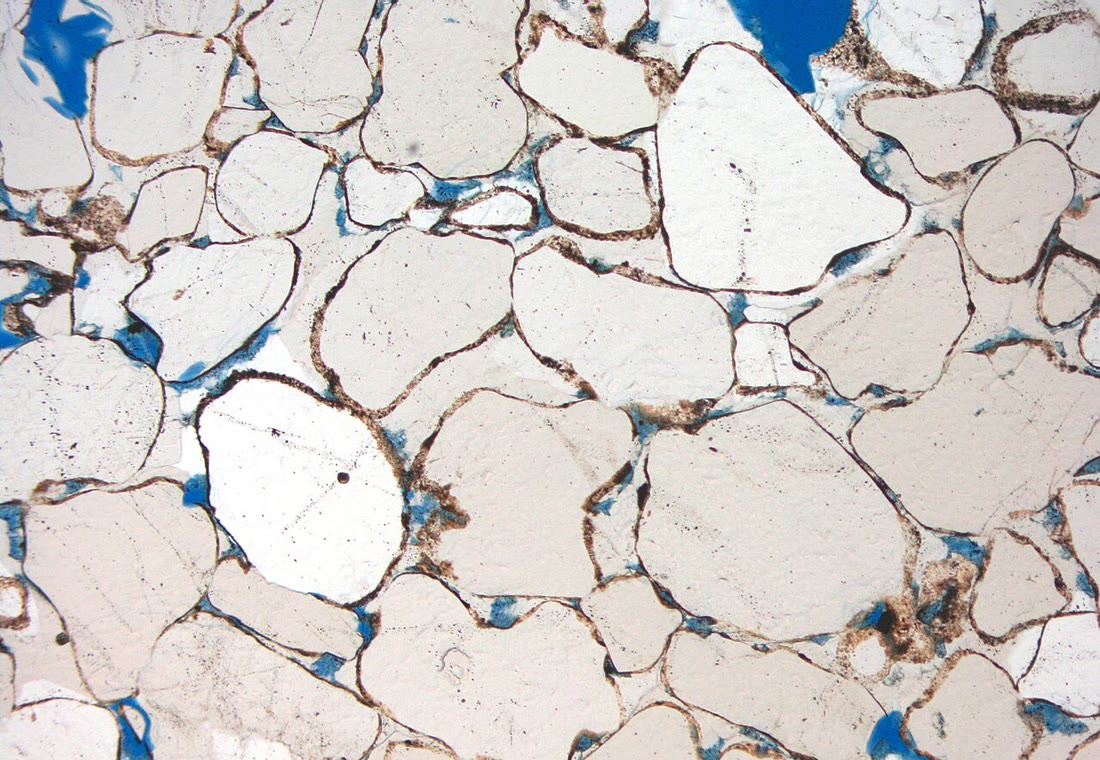
\includegraphics[width=0.62\linewidth]{images/book3/b1-quartz-overgrowths.jpg}

{\small A \omterm{def:b1:field-lab-methods-1:thin-section}{thin section} of quartz sandstone, the Potsdam Sandstone (Cambrian) of
New York State, in \omterm{def:b1:field-lab-methods-1:microscope}{plane-polarised light}. The rounded detrital grains are
outlined by dark rims of dust and clay; the clear quartz outside the rims is
\omterm{def:b1:diagenesis-basins:cement}{cement} that grew on the grains, in optical continuity with them, until the
neighbouring overgrowths met along straight faces. Blue resin fills what is
left of the pores. (M.~C.~Rygel, CC~BY-SA~4.0, via Wikimedia Commons; scale bar
of the original cropped.)}
\label{fig:b1:diagenesis-basins:overgrowths}
\end{omfigure}
% ledger: commons:potsdam

Not every change destroys porosity. Water undersaturated in a \omterm{def:b1:rock-forming-minerals:mineral}{mineral} dissolves
it: grains of \omterm{def:b1:rock-forming-minerals:groups}{feldspar} and of carbonate, and earlier carbonate \omterm{def:b1:diagenesis-basins:cement}{cements}, can be
removed and leave a secondary porosity, pores shaped like the grains they
replace. \omterm{def:b1:weathering-clays:clay-mineral}{Clay minerals} grow in the pores in turn, as coats on the grains or as
crystals that fill the pores and narrow the passages between them, lowering the
permeability. The \omterm{def:b1:rock-forming-minerals:mineral}{minerals} of the sediment change too: the
aragonite of shells and of the \omterm{def:b1:chemical-biogenic-sediments:factory}{carbonate factory} reverts to calcite, which is
stable at the surface, and calcite in the presence of magnesium-bearing water
may become dolomite.
% ledger: og:diagenesis

The replacement of calcite by dolomite, dolomitisation, is a reaction with
magnesium from the water,
\[
  \ce{2 CaCO3 + Mg^2+ -> CaMg(CO3)2 + Ca^2+},
\]
and it changes the volume of the solid.

\begin{proposition}[Dolomitisation creates porosity]\label{prop:b1:diagenesis-basins:dolomite}
If two moles of calcite of density $\rho_c$ are replaced by one mole of dolomite
of density $\rho_d$, the volume of the solid decreases by the fraction
\[
  1 - \frac{M_d/\rho_d}{2M_c/\rho_c},
\]
where $M_c$ and $M_d$ are the molar masses. With $\rho_c = \qty{2.71}{g.cm^{-3}}$
and $\rho_d = \qty{2.84}{g.cm^{-3}}$ this fraction is \qty{12.1}{\percent}.
\end{proposition}

\begin{proof}
The molar volume of a \omterm{def:b1:rock-forming-minerals:mineral}{mineral} is its molar mass divided by its density. Two
moles of calcite occupy $2M_c/\rho_c$ and one of dolomite $M_d/\rho_d$; the
fraction lost is one minus their ratio. With $M_c = \qty{100.09}{g.mol^{-1}}$
and $M_d = \qty{184.40}{g.mol^{-1}}$ the two volumes are
$2\times\qty{36.93}{cm^3} = \qty{73.86}{cm^3}$ and \qty{64.93}{cm^3}, and
$1 - 64.93/73.86 = \num{0.121}$.
\end{proof}

If the outer volume of the rock does not change, the solid lost is pore space
gained: a limestone of porosity \num{0.10} replaced mole for mole by dolomite has
a porosity of about \num{0.21}. The reaction needs a great deal of magnesium,
which seawater holds at about \qty{1.28}{g} a kilogram; it is favoured where
brines or seawater flow through the rock for a long time
(\cref{exo:b1:diagenesis-basins:12}).
% ledger: hom:calcite, webmineral:others, teos10:reference-composition, teos10:reference-salinity

\omterm{def:b1:diagenesis-basins:diagenesis}{Diagenesis} follows the history of the sediment. Just after deposition, near the
surface, the pore water is still that of the sea, the lake or the rain:
sediments are burrowed, cemented early on the sea floor or in the soil, and
aragonite turns to calcite. With burial and heating, \omterm{def:b1:diagenesis-basins:compaction}{compaction}, pressure
solution and quartz \omterm{def:b1:diagenesis-basins:cement}{cement} dominate. If the basin is
later uplifted and eroded, fresh water from the surface flows back into the
rocks, and dissolves carbonate and \omterm{def:b1:rock-forming-minerals:groups}{feldspar} again. A \omterm{def:b1:field-lab-methods-1:thin-section}{thin section} records the
order of these events: a \omterm{def:b1:diagenesis-basins:cement}{cement} that fills the pore left by a dissolved grain is
younger than the dissolution, an overgrowth broken by \omterm{def:b1:diagenesis-basins:compaction}{compaction} older than the
\omterm{def:b1:diagenesis-basins:compaction}{compaction}.

\section{Sedimentary basins}\label{sec:b1:diagenesis-basins:basins}

Sediment kilometres thick accumulates only where the floor keeps sinking.

\begin{definition}[Sedimentary basin]\label{def:b1:diagenesis-basins:basin}
A \emph{sedimentary basin}\index{sedimentary basin} is a region of the Earth's
surface where the \omterm{def:b1:layered-earth:layers}{crust} has subsided for a long time, a few million to a few
hundred million years, and where the space so created has been filled with
sediment, hundreds of metres to many kilometres thick.
\end{definition}

\begin{definition}[Subsidence, tectonic subsidence]\label{def:b1:diagenesis-basins:subsidence}
The \emph{subsidence}\index{subsidence} of a basin is the downward motion of its
basement, the surface on which its sediments rest, measured relative to a fixed
reference such as the centre of the Earth. Its \emph{tectonic
subsidence}\index{tectonic subsidence} is the part due to the processes that
make the basin, as distinct from the extra sinking caused by the weight of the
sediment and water that fill it; it is measured by the subsidence the basement
would have had under water alone.
\end{definition}

What makes the floor sink is the setting of the basin in the plate (figure
below).

\begin{description}
  \item[Rift basins.] \omterm{def:b1:faults-folds-fabrics:fault-types}{Normal faults} stretch the crust, and blocks drop between
        them (\cref{ch:b1:rifts-ridges-margins}). The basins are narrow and
        asymmetric, \omterm{def:b1:rifts-ridges-margins:rift}{half-grabens} filled fastest against their border fault. The
        oilfields of the North Sea lie in the structures of its Viking and
        Central Grabens, buried under younger sediments. When the stretching
        stops, the thinned and heated \omterm{def:b1:layered-earth:lithosphere}{lithosphere} cools, contracts and goes on
        sinking, slowly, over tens of millions of years. The central North Sea,
        whose last major stretching ended in the mid-Cretaceous, then sank as a
        broad, saucer-shaped basin, filled successively by chalks, sandstones
        and, through most of the Tertiary, shales and mudstones; its basement,
        loaded by water alone, would have sunk \qtyrange{1100}{1400}{m} in the
        middle.
  \item[\omterm{def:b1:rifts-ridges-margins:passive-margin}{Passive margins}.] Where the rift became an ocean, the same cooling
        makes each margin sink after break-up, and a wedge of sediment
        thickening towards the ocean builds out over the old rift basins.
  \item[Foreland basins.] In front of a thrust belt, the weight of the stacked
        thrust sheets bends the \omterm{def:b1:layered-earth:lithosphere}{lithosphere} down, by \omterm{def:b1:isostasy-gravity:isostasy}{isostasy}, into a basin
        deepest against the belt and filled by the debris eroded from it. Most
        of the Cretaceous rocks of western Canada were laid down in such a basin
        in front of the Rocky Mountains.
  \item[Intracratonic basins.] In the interior of old continents, far from any
        plate boundary, broad round or oval regions have sunk slowly for very
        long times. The Paris Basin is the centre of such a structural
        depression, between the old massifs of Brittany, the Massif Central and
        the Vosges and Ardennes.
  \item[Strike-slip basins.] Where a \omterm{def:b1:faults-folds-fabrics:fault-types}{strike-slip fault} steps aside in the
        sense that pulls its walls apart --- a releasing bend --- a parallelogram
        of \omterm{def:b1:layered-earth:layers}{crust} subsides between the two fault strands: a pull-apart basin, such
        as those of the Los Angeles region along the San Andreas system.
\end{description}
% ledger: ws:basins, sc80:north-sea, britannica:paris-basin

Why the \omterm{def:b1:layered-earth:lithosphere}{lithosphere} sinks in each setting, at what rate, and how the basins
compare, is the subject of the Year~2 volume; here they are told apart by where
they lie and by the shape of their fill.

\begin{omfigure}
\begin{tikzpicture}[font=\scriptsize, line join=round]
% (a) rift: a half-graben
\begin{scope}
  \fill[lith granite] (0,0) -- (0,1.6) -- (1.4,1.6) -- (2.2,0.2) -- (5.0,1.0) -- (5.0,0) -- cycle;
  \fill[lith shale] (1.4,1.6) -- (2.2,0.2) -- (5.0,1.0) -- (5.0,1.6) -- cycle;
  \fill[lith sandstone] (1.4,1.6) -- (1.75,0.99) -- (5.0,1.25) -- (5.0,1.6) -- cycle;
  \draw[normal fault, thick] (1.4,1.6) -- (2.3,0.0);
  \draw[black!70] (0,1.6) -- (5.0,1.6);
  \node[anchor=south west] at (0,1.65) {(a) rift: a half-graben};
  \node[fill=white, fill opacity=0.8, text opacity=1, inner sep=1pt] at (3.9,0.3) {basement};
  \node[fill=white, fill opacity=0.8, text opacity=1, inner sep=1pt] at (0.65,0.8) {footwall};
\end{scope}
% (b) passive margin: a seaward-thickening wedge over thinned crust
\begin{scope}[xshift=6.6cm]
  \fill[lith sea] (2.0,1.6) -- (5.0,1.6) -- (5.0,0.75) -- (3.6,0.95) -- cycle;
  \fill[lith granite] (0,0) -- (0,1.2) -- (2.0,1.0) -- (3.6,0.35) -- (5.0,0.05) -- (5.0,0) -- cycle;
  \fill[lith shale] (0,1.2) -- (2.0,1.0) -- (3.6,0.35) -- (5.0,0.05) -- (5.0,0.75) -- (3.6,0.95) -- (2.0,1.6) -- (0,1.6) -- cycle;
  \draw[black!70] (0,1.6) -- (2.0,1.6) -- (3.6,0.95) -- (5.0,0.75);
  \draw[blue!60!black, thick] (2.0,1.6) -- (5.0,1.6);
  \node[anchor=south west] at (0,1.65) {(b) passive margin};
  \node[fill=white, fill opacity=0.8, text opacity=1, inner sep=1pt] at (1.0,0.45) {thinned continental crust};
  \node[anchor=north east] at (5.0,1.58) {ocean};
\end{scope}
% (c) foreland basin: asymmetric, deepest against the thrust belt
\begin{scope}[yshift=-3.3cm]
  \fill[lith granite] (0,0) -- (0,0.55) -- (5.0,1.35) -- (5.0,0) -- cycle;
  \fill[lith sandstone] (0,0.55) -- (5.0,1.35) -- (5.0,1.6) -- (0,1.6) -- cycle;
  \fill[lith conglomerate] (1.0,1.6) -- (3.6,1.6) -- (1.0,1.0) -- cycle;
  \fill[omLithSchist, draw=black!70] (0,0.95) -- (1.9,1.6) -- (1.3,1.95) -- (0.4,2.25) -- (0,2.3) -- cycle;
  \draw[thrust fault] (0,0.95) -- (1.9,1.6);
  \draw[thrust fault] (0,1.55) -- (1.15,1.95);
  \draw[black!70] (1.9,1.6) -- (5.0,1.6);
  \node[anchor=south west] at (2.0,1.65) {(c) foreland basin};
  \node[anchor=south west, inner sep=1pt] at (0.25,2.3) {thrust belt};
  \node[fill=white, fill opacity=0.8, text opacity=1, inner sep=1pt] at (3.9,0.35) {basement};
\end{scope}
% (d) intracratonic basin: a broad sag, layers thickening to the centre
\begin{scope}[xshift=6.6cm, yshift=-3.3cm]
  \fill[lith granite] (0,0) -- (0,1.5) .. controls (1.6,1.1) and (2.0,0.3) .. (2.5,0.3) .. controls (3.0,0.3) and (3.4,1.1) .. (5.0,1.5) -- (5.0,0) -- cycle;
  \fill[lith limestone] (0,1.5) .. controls (1.6,1.1) and (2.0,0.3) .. (2.5,0.3) .. controls (3.0,0.3) and (3.4,1.1) .. (5.0,1.5) -- (5.0,1.6) -- (0,1.6) -- cycle;
  \fill[lith shale] (0.6,1.6) .. controls (1.6,1.35) and (2.1,0.85) .. (2.5,0.85) .. controls (2.9,0.85) and (3.4,1.35) .. (4.4,1.6) -- cycle;
  \fill[lith sandstone] (1.3,1.6) .. controls (1.9,1.5) and (2.2,1.3) .. (2.5,1.3) .. controls (2.8,1.3) and (3.1,1.5) .. (3.7,1.6) -- cycle;
  \draw[black!70] (0,1.6) -- (5.0,1.6);
  \node[anchor=south west] at (0,1.65) {(d) intracratonic basin};
  \node[fill=white, fill opacity=0.8, text opacity=1, inner sep=1pt] at (4.2,0.4) {basement};
\end{scope}
\end{tikzpicture}

{\small Four kinds of \omterm{def:b1:diagenesis-basins:basin}{sedimentary basin} in cross-section (schematic, not to
scale; vertical scale exaggerated). (a)~A rift: the fill thickens against the
border fault of a \omterm{def:b1:rifts-ridges-margins:rift}{half-graben}. (b)~A \omterm{def:b1:rifts-ridges-margins:passive-margin}{passive margin}: a wedge of sediment
thickening towards the ocean over thinned continental \omterm{def:b1:layered-earth:layers}{crust}. (c)~A foreland
basin, deepest against the thrust belt whose weight bends it down, and fed by
its debris, coarsest (conglomerate) near the belt; the belt overrides the edge
of its own basin. (d)~An intracratonic basin: a broad sag whose layers thicken
towards the centre.}
\label{fig:b1:diagenesis-basins:types}
\end{omfigure}

\begin{inthefield}[How basins are known]
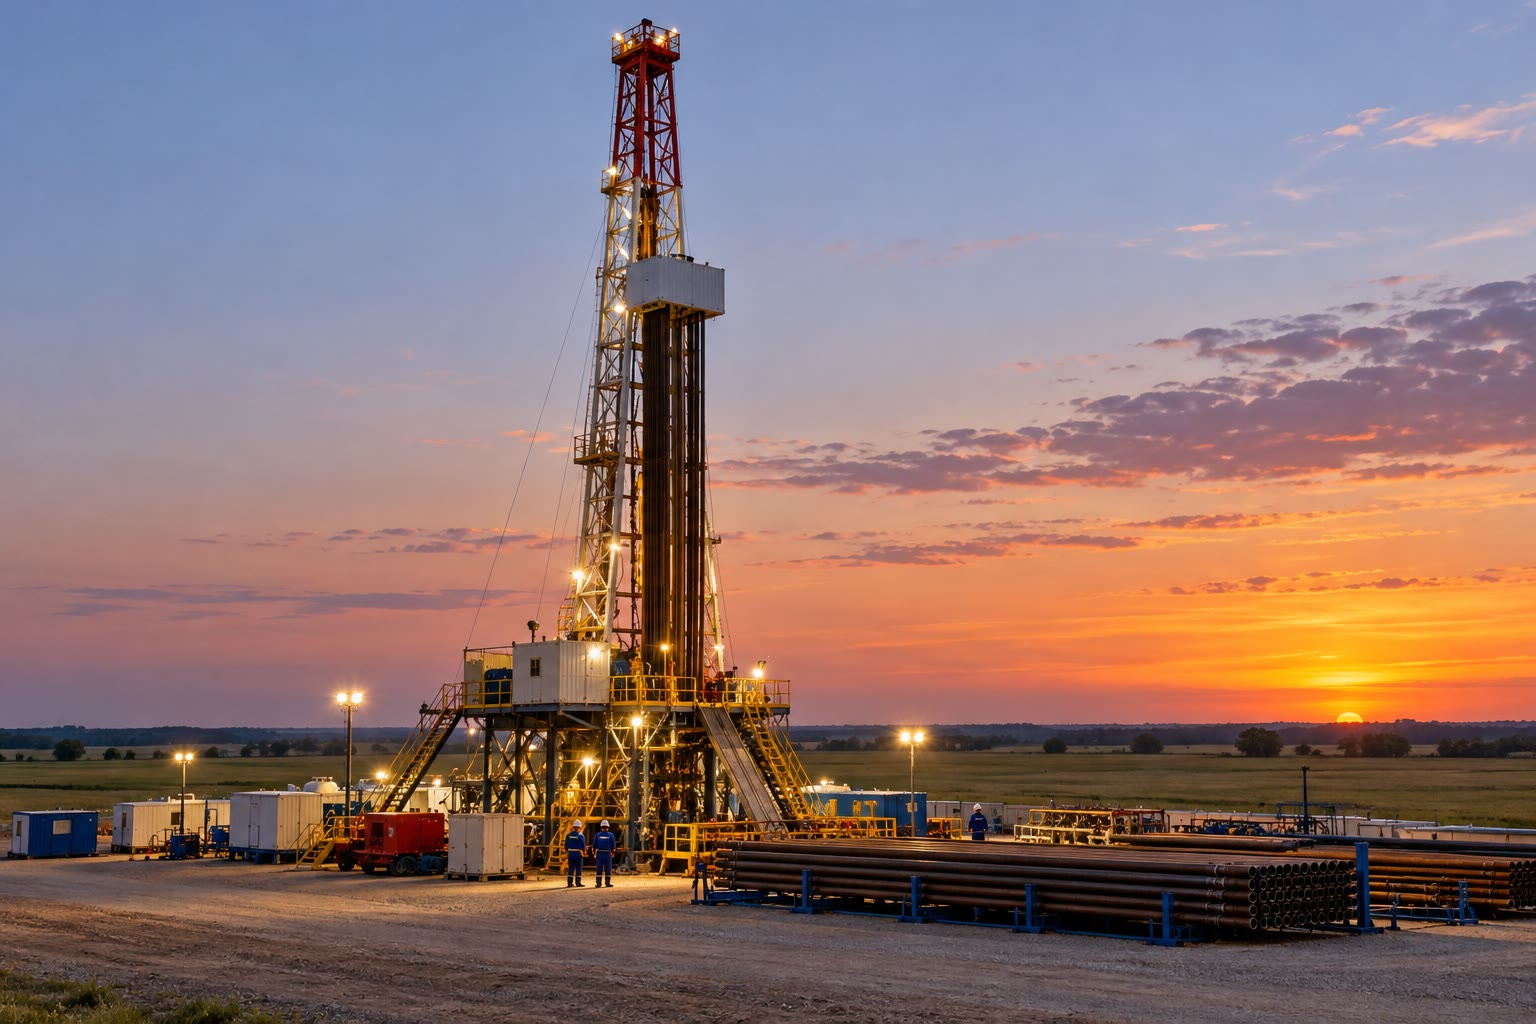
\includegraphics[width=0.3\linewidth]{images/book3/ai/b1-drilling-rig.jpg}\hfill
\begin{minipage}[b]{0.67\linewidth}
Almost everything known about the deep fill of a basin comes from the search
for oil, gas and water. Seismic reflection surveys image its layers and its
faults over thousands of square kilometres; wells sample it at a point. A well
returns the chips of rock cut by the bit, at intervals cores, and continuous
logs of the physical properties of the rocks around the hole, from which the
porosity is read metre by metre. The porosity--depth curves of \omterm{prop:b1:diagenesis-basins:athy}{Athy's law}, and
the \omterm{def:b1:diagenesis-basins:subsidence}{subsidence} histories of basins, were first built from such wells.
\end{minipage}

\smallskip
{\small A land drilling rig at dusk, pipe stacked on racks in the foreground (AI
illustration).}
\end{inthefield}
% ledger: sc80:north-sea

\section{Subsidence, accommodation and sea level}\label{sec:b1:diagenesis-basins:accommodation}

Sediment can pile up only where there is room for it below the level at which
it would be moved on. In the sea that level is close to sea level, and the room
is a matter of two motions: of the floor, and of the sea surface.

\begin{definition}[Accommodation]\label{def:b1:diagenesis-basins:accommodation}
The \emph{accommodation}\index{accommodation} at a point of a basin is the space
available for sediment to accumulate there: the vertical distance from the top
of the sediment to sea level, the base level of marine deposition. The
accommodation created in an interval of time is the increase of the distance
from a datum attached to the basement to sea level.
\end{definition}

\begin{definition}[Eustasy, relative sea level]\label{def:b1:diagenesis-basins:eustasy}
\emph{Eustasy}\index{eustasy} is the change of the level of the world ocean
measured relative to a fixed reference, the centre of the Earth, caused by a
change in the volume of water in the ocean or in the volume of the ocean
basins; it is the same everywhere. The \emph{relative sea
level}\index{relative sea level} at a place is the height of the sea surface
above a datum attached to the basement there; it changes by eustasy and by the
vertical motion of the ground.
\end{definition}

\begin{proposition}[The accommodation budget]\label{prop:b1:diagenesis-basins:budget}
In an interval of time, let $\Delta E$ be the eustatic rise of sea level and $S$
the \omterm{def:b1:diagenesis-basins:subsidence}{subsidence} of the basement (both positive upwards for the sea, downwards for
the floor). The \omterm{def:b1:diagenesis-basins:accommodation}{accommodation} created is
\[
  \Delta A = \Delta E + S ,
\]
and it is shared between the thickness of sediment added above the datum,
$\Delta T$, and the deepening of the water, $\Delta W$:
$\Delta E + S = \Delta T + \Delta W$.
\end{proposition}

\begin{proof}
Measure heights from the fixed reference. Let $e$ be the height of the sea
surface, $b$ that of the datum, $T$ the thickness of sediment above the datum,
and $W$ the depth of water above the sediment, so that $e = b + T + W$. The
\omterm{def:b1:diagenesis-basins:eustasy}{relative sea level} is $R = e - b = T + W$. Over the interval, $\Delta e =
\Delta E$ and $\Delta b = -S$, so $\Delta R = \Delta E + S$; and $\Delta R =
\Delta T + \Delta W$.
\end{proof}

A sea floor kept at a constant depth ($\Delta W = 0$) is filled exactly as fast
as \omterm{def:b1:diagenesis-basins:accommodation}{accommodation} is created; one that shallows is filled faster, and the
shoreline moves out to sea; one that deepens is starved. $\Delta T$ is the
change of thickness of the whole pile above the datum: it counts the new
sediment laid down, minus the thinning of the older sediments below as they
compact, so \omterm{def:b1:diagenesis-basins:compaction}{compaction} itself makes room for more sediment (figure below).

\begin{omfigure}
\begin{tikzpicture}[font=\footnotesize, >=Stealth]
\def\col#1#2#3#4#5{% x, datum, sediment top, sea, label
  \fill[lith granite] (#1,0.2) rectangle ++(1.4,#2-0.2);
  \fill[lith shale] (#1,#2) rectangle ++(1.4,#3-#2);
  \fill[lith sea] (#1,#3) rectangle ++(1.4,#4-#3);
  \draw[black!70] (#1,#2) -- ++(1.4,0);
  \draw[blue!60!black, thick] (#1-0.2,#4) -- ++(1.8,0);
  \node[anchor=north] at (#1+0.7,0.15) {#5};}
\draw[black!60, dash dot] (-0.6,0.9) -- (8.6,0.9) node[anchor=west, align=left] {fixed\\ reference};
\col{0}{1.5}{3.0}{3.6}{time $t_1$}
\col{4.4}{1.0}{3.4}{3.9}{time $t_2$}
% eustasy
\draw[<->, omThm] (3.0,0.9) -- (3.0,3.6) node[midway, fill=white, inner sep=1pt] {$e_1$};
\draw[<->, omThm] (7.4,0.9) -- (7.4,3.9) node[midway, fill=white, inner sep=1pt] {$e_2$};
% subsidence of the datum
\draw[dashed, black!60] (1.4,1.5) -- (4.4,1.5);
\draw[->, thick] (4.2,1.5) -- (4.2,1.0) node[midway, anchor=east] {$S$};
% relative sea level
\draw[<->] (-0.35,1.5) -- (-0.35,3.6) node[midway, anchor=east] {$R_1$};
\draw[<->] (6.05,1.0) -- (6.05,3.9) node[midway, anchor=west] {$R_2$};
\node[anchor=west] at (1.5,2.25) {$T_1$};
\node[anchor=west] at (1.5,3.3) {$W_1$};
\node at (5.1,2.2) {$T_2$};
\node at (5.1,3.65) {$W_2$};
\node[anchor=south, align=center, blue!60!black] at (5.1,3.95) {sea level};
\node[anchor=west, align=left, font=\scriptsize] at (8.6,2.4) {$R = e - b = T + W$\\[2pt] $\Delta R = \Delta E + S$\\ $\phantom{\Delta R} = \Delta T + \Delta W$};
\end{tikzpicture}

{\small \omterm{def:b1:diagenesis-basins:accommodation}{Accommodation} at one place at two times (schematic). Between $t_1$ and
$t_2$ sea level rises by $\Delta E = e_2 - e_1$ above the fixed reference and
the basement subsides by $S$: the \omterm{def:b1:diagenesis-basins:eustasy}{relative sea level} $R$ grows by $\Delta E + S$,
the \omterm{def:b1:diagenesis-basins:accommodation}{accommodation} created, which is shared between more sediment ($T_2 > T_1$)
and a change of water depth (here a slight shallowing, $W_2 < W_1$).}
\label{fig:b1:diagenesis-basins:accommodation}
\end{omfigure}

A basin does not sink by its \omterm{def:b1:diagenesis-basins:subsidence}{tectonic subsidence} alone: the sediment that fills
it is a load, and the \omterm{def:b1:layered-earth:lithosphere}{lithosphere} sinks further under it.

\begin{proposition}[Sediment loading amplifies subsidence]\label{prop:b1:diagenesis-basins:loading}
In local (Airy) \omterm{def:b1:isostasy-gravity:isostasy}{isostasy} over a \omterm{def:b1:layered-earth:layers}{mantle} of density $\rho_m$, a basin whose
basement, loaded by water of density $\rho_w$ alone, would lie at the depth $Y$
below sea level holds, when filled to sea level with sediment of mean density
$\rho_s$, the thickness
\[
  h = Y\,\frac{\rho_m - \rho_w}{\rho_m - \rho_s}
\]
of sediment. On land, filled to the level of the surroundings with air above,
the factor is $\rho_m/(\rho_m - \rho_s)$.
\end{proposition}

\begin{proof}
Compare the two columns with the same \omterm{def:b1:layered-earth:lithosphere}{lithosphere}, of mass $M$ per unit area and
thickness $L$, down to a \omterm{def:b1:isostasy-gravity:isostasy}{compensation depth} $z_c$ below both. The water-loaded
column holds $\rho_w Y + M + \rho_m(z_c - Y - L)$; the sediment-filled one
$\rho_s h + M + \rho_m(z_c - h - L)$. By
\cref{prop:b1:isostasy-gravity:equal-mass} the two masses are equal, so
$\rho_w Y - \rho_m Y = \rho_s h - \rho_m h$, that is $h(\rho_m - \rho_s) =
Y(\rho_m - \rho_w)$. With air in place of water, $\rho_w$ is replaced by zero.
\end{proof}

With $\rho_m = \qty{3300}{kg.m^{-3}}$, $\rho_w = \qty{1030}{kg.m^{-3}}$ and
sediment of mean density \qty{2300}{kg.m^{-3}}, the factor is
$2270/1000 = \num{2.27}$: a basin whose \omterm{def:b1:diagenesis-basins:subsidence}{tectonic subsidence} would make room for
\qty{1}{km} of water holds \qty{2.27}{km} of sediment. On land the factor would
be $3300/1000 = \num{3.3}$. The density of the fill is not constant: it grows as
the sediment compacts, and the factor with it, so that turning a sediment
thickness into a \omterm{def:b1:diagenesis-basins:subsidence}{tectonic subsidence} requires the \omterm{def:b1:diagenesis-basins:compaction}{decompaction} of each layer,
time step by time step. That procedure, backstripping, belongs to the Year~2
volume.

Sea level itself is far from fixed. At the Last Glacial Maximum, ice sheets
covered much of North America and northern Europe, and the water locked in them
had been taken from the ocean. Corrected for the response of the solid Earth to
the changing loads of ice and water, the observations of former shorelines give
a sea level that fell quickly by about \qty{40}{m} some \num{30000} years ago
and then slowly, to \qty{134}{m} below today's, from \qtyrange{29}{21}{\ka};
the grounded ice then held about \qty{52e6}{km^3} more than today. The figure
of \qty{125}{m} often quoted is smaller because it is usually not corrected for
these isostatic effects. Deglaciation came mainly between about \qty{16.5}{\ka}
and \qty{8.2}{\ka}, at an average of \qty{12}{m} per thousand years, and at
\qty{40}{mm} a year or more between \qty{14.5}{\ka} and \qty{14.0}{\ka}.
% ledger: lambeck:lgm, lambeck:deglaciation

Older lowstands are read from the oxygen isotopes of foraminifera in deep-sea
cores, which record the volume of ice on land. Stacking seven such
reconstructions over the last \num{430000} years, and five over the last
\num{800000}, averages out the errors of each; scaled to the Holocene and to the
last glacial lowstand, the stack carries an uncertainty of
\qtyrange{9}{12}{m} (figure below). It shows the glacial cycles as a saw-tooth:
slow falls of sea level, each ended by a fast rise --- five times in the last
\num{800000} years a rise of more than \qty{100}{m} in less than \num{20000}
years. \omterm{def:b1:diagenesis-basins:eustasy}{Eustasy} on this scale moves the shoreline back and forth across the
continental shelves.
% ledger: spratt:stack, data:b3-sealevel-stack

\begin{omfigure}
\begin{tikzpicture}[font=\footnotesize]
\begin{axis}[width=16cm, height=4.8cm, xmin=0, xmax=800, ymin=-150, ymax=40,
    x dir=reverse, xlabel={age (thousands of years before present)}, xlabel style={yshift=2pt},
    ylabel={sea level (m)}, ytick={-150,-100,-50,0},
    title={(a) the last \num{800000} years (five records)}, title style={font=\footnotesize},
    axis on top]
  \addplot[draw=none, name path=hi] table[x=age, y=hi] {figdata/out/bachelor-1-sea_level-long.dat};
  \addplot[draw=none, name path=lo] table[x=age, y=lo] {figdata/out/bachelor-1-sea_level-long.dat};
  \addplot[omThm!25] fill between[of=hi and lo];
  \addplot[thin, omThm] table[x=age, y=sl] {figdata/out/bachelor-1-sea_level-long.dat};
  \draw[black!50, densely dotted] (axis cs:0,0) -- (axis cs:800,0);
\end{axis}
\end{tikzpicture}

\medskip
\begin{tikzpicture}[font=\footnotesize]
\begin{axis}[width=16cm, height=4.8cm,
    xmin=0, xmax=140, ymin=-160, ymax=40, x dir=reverse,
    xlabel={age (thousands of years before present)}, ylabel={sea level (m)},
    ytick={-150,-100,-50,0},
    title={(b) the last \num{140000} years (seven records)}, title style={font=\footnotesize},
    axis on top]
  \addplot[draw=none, name path=hi] table[x=age, y=hi] {figdata/out/bachelor-1-sea_level-short.dat};
  \addplot[draw=none, name path=lo] table[x=age, y=lo] {figdata/out/bachelor-1-sea_level-short.dat};
  \addplot[omThm!25] fill between[of=hi and lo];
  \addplot[thick, omThm] table[x=age, y=sl] {figdata/out/bachelor-1-sea_level-short.dat};
  \draw[black!50, densely dotted] (axis cs:0,0) -- (axis cs:140,0);
  \addplot[only marks, mark=*, mark size=1.6pt, black] coordinates {(21,-134)};
  \draw[black!60, thin] (axis cs:21,-131) -- (axis cs:21,-46);
  \node[anchor=south, font=\scriptsize, fill=white, inner sep=1pt] at (axis cs:36,-46) {\qty{-134}{m} at \qty{21}{\ka} from shorelines (Lambeck et al.\ 2014)};
\end{axis}
\end{tikzpicture}

{\small Global sea level relative to today from the stack of Spratt and
Lisiecki (2016): the first principal component of five reconstructions from
deep-sea cores over \num{800000} years (a) and of seven over the last
\num{140000} (b), with its one-standard-deviation band. The lowest value of the
stack, \qty{-130}{m} at \qty{24}{\ka}, lies within that band of the
\qty{-134}{m} found from former shorelines (dot); the last interglacial stands
about \qty{3}{m} above today at \qty{121}{\ka}. Data: NOAA NCEI World Data
Service for Paleoclimatology.}
\label{fig:b1:diagenesis-basins:sea-level}
\end{omfigure}
% computed in figdata/bachelor-1/sea_level.py; ledger: data:b3-sealevel-stack, spratt:stack, lambeck:lgm

Over the life of a basin such swings are brief. A glacial fall of more than
\qty{100}{m} in a few tens of thousands of years is fast and large compared with
\omterm{def:b1:diagenesis-basins:subsidence}{tectonic subsidence}, which adds up to a kilometre or more only over tens of
millions of years; but the glacial swings stay within a range of about
\qty{150}{m}, so that in the thick fill of a basin \omterm{def:b1:diagenesis-basins:subsidence}{subsidence} makes most of the
room, and \omterm{def:b1:diagenesis-basins:eustasy}{eustasy} sets the rhythm of its layers.
% ledger: data:b3-sealevel-stack, sc80:north-sea

\section{Exercises}

\begin{exercise}[$\star$]\label{exo:b1:diagenesis-basins:1}
With the parameters of \cref{tab:b1:diagenesis-basins:athy}, compute the
porosity of sandstone and of shale at \qty{2000}{m}. At what depth has the
porosity of each fallen to half its surface value?
% ledger: pybacktrack:compaction
\end{exercise}

\begin{exercise}[$\star$]\label{exo:b1:diagenesis-basins:2}
During an interval of time, sea level rises by \qty{30}{m} by \omterm{def:b1:diagenesis-basins:eustasy}{eustasy}, the
basement of a shelf subsides by \qty{50}{m}, and \qty{60}{m} of sediment are
added above a datum on the basement. With
\cref{prop:b1:diagenesis-basins:budget}, compute the \omterm{def:b1:diagenesis-basins:accommodation}{accommodation} created and
the change of water depth. Does the shelf deepen or shallow?
\end{exercise}

\begin{exercise}[$\star$]\label{exo:b1:diagenesis-basins:3}
A basin's \omterm{def:b1:diagenesis-basins:subsidence}{tectonic subsidence} would make room for \qty{1.0}{km} of water. With
$\rho_m = \qty{3300}{kg.m^{-3}}$ and $\rho_w = \qty{1030}{kg.m^{-3}}$, how
thick is the sediment that fills it to sea level if its mean density is
\qty{2300}{kg.m^{-3}}? \qty{2500}{kg.m^{-3}}? Why does a denser fill give a
thicker one?
\end{exercise}

\begin{exercise}[$\star$]\label{exo:b1:diagenesis-basins:4}
Calcite has the molar mass \qty{100.09}{g.mol^{-1}} and the density
\qty{2.71}{g.cm^{-3}}; dolomite \qty{184.40}{g.mol^{-1}} and
\qty{2.84}{g.cm^{-3}}. (a)~Compute the molar volume of each. (b)~By what
fraction does the volume of the solid change when two moles of calcite become
one mole of dolomite? (c)~A limestone of porosity \num{0.10} is dolomitised
mole for mole without change of its outer volume. What is its new porosity?
% ledger: hom:calcite, webmineral:others
\end{exercise}

\begin{exercise}[$\star\star$]\label{exo:b1:diagenesis-basins:5}
A shale occupies the top \qty{1000}{m} of a basin. (a)~Compute its solid
thickness and its mean porosity. (b)~It is buried until its top lies at
\qty{2000}{m}. Using \cref{met:b1:diagenesis-basins:decompaction} with the top
moved down instead of up, find its new thickness and its mean porosity.
(c)~How much water has each square metre of the shale expelled?
% ledger: pybacktrack:compaction
\end{exercise}

\begin{exercise}[$\star\star$]\label{exo:b1:diagenesis-basins:6}
A sandstone lies between \qty{2500}{m} and \qty{2800}{m}. (a)~Compute its solid
thickness. (b)~Decompact it to the surface with
\cref{met:b1:diagenesis-basins:decompaction}, writing down each Newton step
from $b_0 = \qty{300}{m}$. (c)~By what factor has burial thinned it?
% ledger: pybacktrack:compaction
\end{exercise}

\begin{exercise}[$\star\star$]\label{exo:b1:diagenesis-basins:7}
At the Last Glacial Maximum the grounded ice held about \qty{52e6}{km^3} more
than today. Take the density of ice \qty{916.7}{kg.m^{-3}}, that of meltwater
\qty{1000}{kg.m^{-3}}, and the area of today's ocean
\qty{361.84e6}{km^2}. (a)~What fall of sea level does this ice represent?
(b)~Compare with the \qty{134}{m} found from former shorelines. (c)~What ocean
area would give exactly \qty{134}{m}, and why was the glacial ocean smaller?
% ledger: lambeck:lgm, iapws:ice-density, charette:ocean-volume
\end{exercise}

\begin{exercise}[$\star\star$]\label{exo:b1:diagenesis-basins:8}
The sea-level stack gives \qty{-98.1}{m} at \qty{16}{\ka} and \qty{-9.1}{m} at
\qty{8}{\ka}. (a)~Compute the mean rate of rise, in metres per thousand years,
and compare it with the \qty{12}{m} per thousand years found from former
shorelines for the main deglaciation. (b)~Between \qty{14.5}{\ka} and
\qty{14.0}{\ka} sea level rose at \qty{40}{mm} a year or more. How many times
the average is that, and how much did sea level rise in those five hundred
years?
% ledger: data:b3-sealevel-stack, lambeck:deglaciation
\end{exercise}

\begin{exercise}[$\star\star$]\label{exo:b1:diagenesis-basins:9}
A shelf lies under \qty{20}{m} of water. Its basement subsides at
\qty{50}{m} per million years. (a)~Over two million years sea level falls by
\qty{40}{m} by \omterm{def:b1:diagenesis-basins:eustasy}{eustasy} while the water depth stays the same. How much
\omterm{def:b1:diagenesis-basins:accommodation}{accommodation} is created, and how much sediment is added? (b)~Sea level then
falls by \qty{120}{m} in \num{20000} years, at the onset of a glaciation, and no
sediment is added. How high above sea level does the former sea floor stand at
the end?
\end{exercise}

\begin{exercise}[$\star\star\star$]\label{exo:b1:diagenesis-basins:10}
(a)~Show that a layer of thickness $h$ at the depth $z$, thin compared with the
decay length $\lambda$, has the thickness $h_0 \approx h\,(1 - \varphi(z))/(1 -
\varphi_0)$ when restored to the surface. (b)~Apply it to \qty{10}{m} of shale
at \qty{3000}{m}, and compare with the exact \omterm{def:b1:diagenesis-basins:compaction}{decompaction}, \qty{23.1}{m}.
(c)~Why is the approximation slightly too large?
% ledger: pybacktrack:compaction
\end{exercise}

\begin{exercise}[$\star\star\star$]\label{exo:b1:diagenesis-basins:11}
A basin is filled to sea level by \qty{3000}{m} of shale, compacted by \omterm{prop:b1:diagenesis-basins:athy}{Athy's
law}, its pores full of water of density \qty{1030}{kg.m^{-3}}. (a)~Compute the
mean porosity and the mean density of the fill. (b)~With
\cref{prop:b1:diagenesis-basins:loading} and $\rho_m =
\qty{3300}{kg.m^{-3}}$, compute the loading factor and the water-loaded
\omterm{def:b1:diagenesis-basins:subsidence}{subsidence} that the fill represents. (c)~Why would taking the density of the
grains, \qty{2700}{kg.m^{-3}}, give a much larger factor, and why would that be
wrong?
% ledger: pybacktrack:compaction
\end{exercise}

\begin{exercise}[$\star\star\star$]\label{exo:b1:diagenesis-basins:12}
A cubic metre of limestone of porosity \num{0.10} is to be dolomitised
completely, mole for mole. Seawater holds \qty{35.165}{g} of salt per kilogram,
of which the mass fraction \num{0.0365} is magnesium (\qty{24.305}{g.mol^{-1}}).
(a)~How many moles of calcite does the cube hold (molar volume from
\cref{exo:b1:diagenesis-basins:4})? (b)~How many moles of magnesium does the
reaction need? (c)~What mass and what volume of seawater
(\qty{1030}{kg.m^{-3}}) must flow through the cube if it gives up all its
magnesium? (d)~What does the answer say about where dolomite forms?
% ledger: teos10:reference-composition, teos10:reference-salinity, hom:calcite
\end{exercise}

\section{Problem: Decompacting a basin's fill}

\begin{problem}[{Weekend problem --- how thick the sediments of a well were when
they were laid down, and how the room for them was made}]
\label{pb:b1:diagenesis-basins:1}
% values: calc/ch23.py; the well, its units, ages and the eustatic changes are invented
A well drilled on a coastal plain, at sea level, passes through three units
before it reaches the basement at \qty{3200}{m}:
\begin{center}
\begin{tabular}{llll}
\hline
unit & lithology & depth today (m) & time of deposition \\
\hline
1 & sandstone & 0--800     & \qtyrange{15}{0}{\Ma} \\
2 & shale     & 800--2600  & \qtyrange{55}{15}{\Ma} \\
3 & chalk     & 2600--3200 & \qtyrange{75}{55}{\Ma} \\
\hline
\end{tabular}
\end{center}
Take the parameters of \cref{tab:b1:diagenesis-basins:athy}, pore water of
density \qty{1030}{kg.m^{-3}}, $g = \qty{9.81}{m.s^{-2}}$, and assume that each
unit compacted by \omterm{prop:b1:diagenesis-basins:athy}{Athy's law}, with its water free to escape, throughout its
history. Microfossils show that the water was shallow, and of the same depth, at
the start and at the end of each interval.

\medskip
\noindent\textbf{Part I --- The column today.}
\begin{enumerate}
  \item Compute the porosity at the top and at the base of each unit.
  \item Compute the mean porosity of each unit.
  \item How much water does each unit hold under one square metre?
  \item Compute the bulk density of each unit, saturated with water, and the
        mean density of the whole column.
  \item Compute the lithostatic and the hydrostatic pressures at the base of the
        column, and the \omterm{def:b1:stress-strain-rheology:lithostatic}{effective stress} there.
  \item At what depth are the porosities of sandstone and shale equal? Which is
        the more porous below it?
\end{enumerate}

\noindent\textbf{Part II --- The grains.}
\begin{enumerate}[resume]
  \item Compute the solid thickness of each unit.
  \item What is the solid thickness of the whole column, and what fraction of
        today's column is water?
  \item Compute, for each unit, the rate of accumulation of grains, in metres
        of solid per million years.
  \item Which unit had the fastest supply of grains? The slowest?
\end{enumerate}

\noindent\textbf{Part III --- The units as they were laid down.}
\begin{enumerate}[resume]
  \item How thick was the sandstone when it was laid down? Why is no
        calculation needed?
  \item Decompact the shale to the surface: how thick was it at \qty{15}{\Ma},
        when its deposition had just ended?
  \item Decompact the chalk to the surface: how thick was it at \qty{55}{\Ma}?
  \item How thick was the chalk at \qty{15}{\Ma}, buried under the shale of the
        previous question?
  \item What was the thickness of the whole column above the basement at
        \qty{55}{\Ma} and at \qty{15}{\Ma}?
  \item Compute the rate of sedimentation of each unit from its thickness
        today, and from its thickness at deposition. Which is the meaningful
        one?
  \item By what fraction has the shale thinned since \qty{15}{\Ma}?
\end{enumerate}

\noindent\textbf{Part IV --- Making room.}
\begin{enumerate}[resume]
  \item Take the top of the basement as datum. With
        \cref{prop:b1:diagenesis-basins:budget}, compute the \omterm{def:b1:diagenesis-basins:accommodation}{accommodation}
        created from \qtyrange{75}{55}{\Ma}, from \qtyrange{55}{15}{\Ma} and
        from \qty{15}{\Ma} to today.
  \item An eustatic curve for the region gives sea level \qty{60}{m} higher at
        \qty{55}{\Ma} than at \qty{15}{\Ma}, and \qty{30}{m} higher at
        \qty{15}{\Ma} than today (assumed values). Compute the \omterm{def:b1:diagenesis-basins:subsidence}{subsidence} of
        the basement in the last two intervals.
  \item Compute the mean rate of \omterm{def:b1:diagenesis-basins:subsidence}{subsidence} in each, in metres per million
        years.
  \item What share of the \omterm{def:b1:diagenesis-basins:subsidence}{subsidence} did \omterm{def:b1:diagenesis-basins:eustasy}{eustasy} have to make up in each
        interval? Did \omterm{def:b1:diagenesis-basins:eustasy}{eustasy} help or hinder the basin's filling?
  \item Of the \omterm{def:b1:diagenesis-basins:accommodation}{accommodation} filled since \qty{15}{\Ma}, how much was made by the
        \omterm{def:b1:diagenesis-basins:compaction}{compaction} of the shale and the chalk below?
  \item Why can the \omterm{def:b1:diagenesis-basins:subsidence}{subsidence} of the basement not be read from the thickness
        of the column today?
  \item What was the thickness of the shale unit when it was laid down?
\end{enumerate}
\end{problem}
